\documentclass[tikz,border=3pt]{standalone}
\usepackage{amsmath,bm}
\usepackage{tikz}
\usetikzlibrary{angles,arrows.meta,calc,quotes}

\definecolor{egocolor}{RGB}{65,145,162}
\definecolor{obstaclecolor}{RGB}{232,112,58}
\definecolor{velocitycolor}{RGB}{50,91,143}
\definecolor{relativecolor}{RGB}{31,122,114}
\definecolor{coursecolor}{RGB}{106,130,158}

\def\vehicleDrawingScale{1}
% Shared vector sedan, facing local +x. Arguments: center, yaw, color, steer.
% The caller defines vehicleDrawingScale; body envelope remains 2.10 x 0.96.
% Styling is illustrative, not a change to the vehicle model or dimensions.
\newcommand{\drawvehicle}[4]{%
    \begin{scope}[shift={(#1)},rotate=#2,scale=\vehicleDrawingScale,
        line join=round,line cap=round]
        \tikzset{carOutline/.style={draw=black!78,line width=0.48pt},
            carDetail/.style={draw=black!55,line width=0.26pt},
            carGlass/.style={carDetail,fill=white!80!#3}}
        % Four separate tires; the front pair follows the steering angle.
        \foreach \wheelY in {-0.515,0.515} {
            \begin{scope}[shift={(-0.515,\wheelY)}]
                \path[fill=black,draw=black,line width=0.25pt,
                    rounded corners=0.5pt] (-0.215,-0.085) rectangle (0.215,0.085);
            \end{scope}
            \begin{scope}[shift={(0.515,\wheelY)},rotate=#4]
                \path[fill=black,draw=black,line width=0.25pt,
                    rounded corners=0.5pt] (-0.215,-0.085) rectangle (0.215,0.085);
            \end{scope}
        }
        % Rounded bumper ends and gently tapered front/rear quarters.
        \path[carOutline,fill=white!40!#3]
            (-1.05,-0.28) .. controls (-1.05,-0.40) and (-0.94,-0.46) .. (-0.79,-0.47)
            .. controls (-0.30,-0.48) and (0.45,-0.48) .. (0.79,-0.45)
            .. controls (0.98,-0.43) and (1.05,-0.32) .. (1.05,-0.18)
            -- (1.05,0.18)
            .. controls (1.05,0.32) and (0.98,0.43) .. (0.79,0.45)
            .. controls (0.45,0.48) and (-0.30,0.48) .. (-0.79,0.47)
            .. controls (-0.94,0.46) and (-1.05,0.40) .. (-1.05,0.28) -- cycle;
        % Hood and trunk seams, with separate bumper lines.
        \draw[carDetail] (0.48,-0.35) .. controls (0.67,-0.38) and (0.86,-0.35) .. (0.94,-0.26)
            .. controls (0.98,-0.12) and (0.98,0.12) .. (0.94,0.26)
            .. controls (0.86,0.35) and (0.67,0.38) .. (0.48,0.35);
        \draw[carDetail] (-0.72,-0.36) -- (-0.92,-0.30)
            .. controls (-0.98,-0.12) and (-0.98,0.12) .. (-0.92,0.30) -- (-0.72,0.36);
        \draw[carDetail] (1.01,-0.15) -- (1.01,0.15);
        \draw[carDetail] (-1.01,-0.23) -- (-1.01,0.23);
        % Front and rear windscreens surround the central roof panel.
        \path[carGlass] (0.19,-0.29) .. controls (0.26,-0.17) and (0.26,0.17) .. (0.19,0.29)
            -- (0.44,0.36) .. controls (0.57,0.18) and (0.57,-0.18) .. (0.44,-0.36) -- cycle;
        \path[carGlass] (-0.45,-0.29) -- (-0.45,0.29) -- (-0.69,0.35)
            .. controls (-0.77,0.16) and (-0.77,-0.16) .. (-0.69,-0.35) -- cycle;
        \path[carDetail,fill=white!60!#3,rounded corners=0.8pt]
            (-0.43,-0.28) -- (0.17,-0.28) -- (0.17,0.28) -- (-0.43,0.28) -- cycle;
        % Side glazing, pillars, door seams, mirrors and lights are symmetric.
        \foreach \side in {-1,1} {
            \begin{scope}[yscale=\side]
                \path[carGlass] (-0.66,0.39) -- (-0.43,0.32) -- (-0.13,0.32)
                    -- (-0.13,0.41) -- cycle;
                \path[carGlass] (-0.08,0.32) -- (0.18,0.32) -- (0.41,0.39)
                    -- (-0.08,0.41) -- cycle;
                \draw[carDetail] (-0.10,0.42) -- (-0.10,0.47);
                \draw[carDetail] (-0.53,0.42) -- (-0.57,0.47);
                \draw[carDetail] (0.34,0.42) -- (0.31,0.47);
                \draw[carDetail] (-0.27,0.445) -- (-0.20,0.445);
                \draw[carDetail] (0.12,0.445) -- (0.19,0.445);
                \path[carDetail,fill=white!60!#3] (0.32,0.43) -- (0.32,0.56)
                    .. controls (0.34,0.61) and (0.43,0.59) .. (0.45,0.55)
                    -- (0.41,0.44) -- cycle;
                \path[carDetail,fill=white] (0.83,0.38) -- (0.96,0.28)
                    -- (0.96,0.19) .. controls (0.90,0.22) and (0.85,0.28) .. (0.83,0.38);
                \path[carDetail,fill=#3!65] (-0.95,0.30) -- (-0.83,0.39)
                    -- (-0.91,0.40) -- (-1.00,0.32) -- cycle;
            \end{scope}
        }
    \end{scope}%
}


% Design critique: keep. Math/diagram logic: schematic; original centers,
% frames, angles and steering are unchanged. Manual visual review confirms
% the inherited angle labels remain separate despite crowding warnings.
\begin{document}
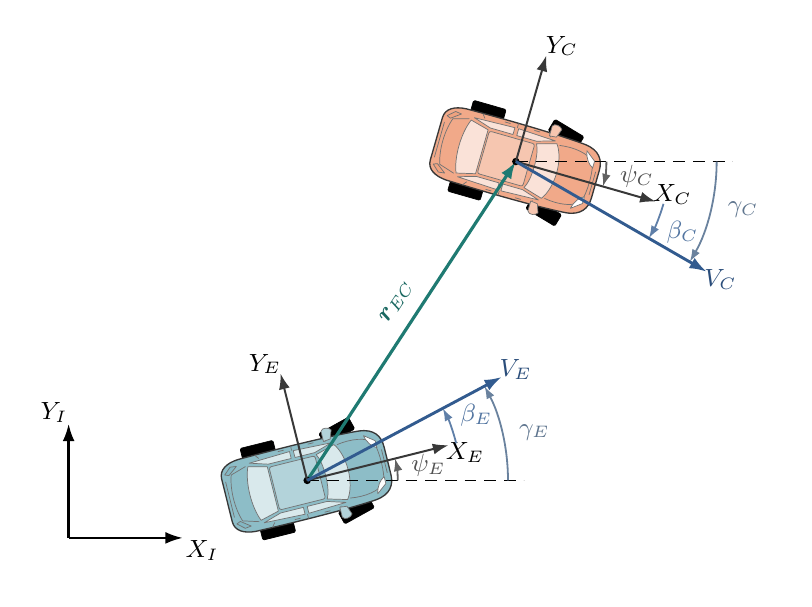
\begin{tikzpicture}[
    font=\sffamily\small,
    >=Latex,
    inertialAxis/.style={
        -{Latex[length=2.2mm,width=1.5mm]},
        draw=black,
        line width=0.85pt
    },
    bodyAxis/.style={
        -{Latex[length=2.0mm,width=1.4mm]},
        draw=black!78,
        line width=0.72pt
    },
    relativeVector/.style={
        -{Latex[length=2.2mm,width=1.5mm]},
        draw=relativecolor,
        line width=1.15pt
    },
    velocityVector/.style={
        -{Latex[length=2.2mm,width=1.5mm]},
        draw=velocitycolor,
        line width=1.05pt
    },
    yawArc/.style={
        -{Latex[length=1.6mm,width=1.1mm]},
        draw=black!62,
        line width=0.65pt
    },
    slipArc/.style={
        -{Latex[length=1.6mm,width=1.1mm]},
        draw=velocitycolor!78,
        line width=0.65pt
    },
    courseArc/.style={
        -{Latex[length=1.6mm,width=1.1mm]},
        draw=coursecolor,
        line width=0.65pt
    },
    mathLabel/.style={
        font=\sffamily\small,
        inner sep=1.2pt,
        text=black
    },
    yawLabel/.style={
        mathLabel,
        text=black!68
    },
    slipLabel/.style={
        mathLabel,
        text=velocitycolor!85
    },
    courseLabel/.style={
        mathLabel,
        text=coursecolor!90!black
    }
]

\path[use as bounding box] (0.20,0.10) rectangle (9.80,7.10);

\coordinate (inertialOrigin) at (0.72,0.62);
\coordinate (egoOrigin) at (3.75,1.35);
\coordinate (obstacleOrigin) at (6.40,5.40);
\def\egoHeading{14}
\def\egoCourse{28}
\def\obstacleHeading{-16}
\def\obstacleCourse{-30}
\def\egoSteer{15}
\def\obstacleSteer{-15}

\drawvehicle{egoOrigin}{\egoHeading}{egocolor}{\egoSteer}
\drawvehicle{obstacleOrigin}{\obstacleHeading}{obstaclecolor}{\obstacleSteer}

% Relative position of the obstacle vehicle in the ego frame.
\draw[relativeVector] (egoOrigin) -- (obstacleOrigin)
    node[mathLabel,pos=0.52,above=1.4mm,sloped,
         text=relativecolor!85!black]
    {$\bm r_{EC}$};

% ---- Ego vehicle -------------------------------------------------------
\path[fill=black] (egoOrigin) circle (1.35pt);

\draw[bodyAxis] (egoOrigin) -- ++(\egoHeading:1.85)
    node[mathLabel,below right=-0.9mm] {$X_E$};
\draw[bodyAxis] (egoOrigin) -- ++(\egoHeading+90:1.40)
    node[mathLabel,above left=-0.6mm] {$Y_E$};
\draw[black,dash pattern=on 1.5mm off 1.0mm]
    (egoOrigin) -- ++(0:2.75);
\draw[yawArc]
    ($(egoOrigin)+(0:1.15)$)
    arc[start angle=0,end angle=\egoHeading,radius=1.15];
\node[yawLabel] at ($(egoOrigin)+(7:1.55)$) {$\psi_E$};
\draw[courseArc]
    ($(egoOrigin)+(0:2.55)$)
    arc[start angle=0,end angle=\egoCourse,radius=2.55];
\node[courseLabel] at ($(egoOrigin)+(12:2.95)$) {$\gamma_E$};
\draw[slipArc]
    ($(egoOrigin)+(\egoHeading:1.95)$)
    arc[start angle=\egoHeading,end angle=\egoCourse,radius=1.95];
\node[slipLabel] at ($(egoOrigin)+(21:2.30)$) {$\beta_E$};
\draw[velocityVector] (egoOrigin) -- ++(\egoCourse:2.80)
    node[mathLabel,above right=-0.9mm,text=velocitycolor!85!black]
    {$V_E$};

% ---- Obstacle vehicle --------------------------------------------------
\path[fill=black] (obstacleOrigin) circle (1.35pt);

\draw[bodyAxis] (obstacleOrigin) -- ++(\obstacleHeading:1.85)
    node[mathLabel,above right=-0.9mm] {$X_C$};
\draw[bodyAxis] (obstacleOrigin) -- ++(\obstacleHeading+90:1.40)
    node[mathLabel,above right=-0.6mm] {$Y_C$};
\draw[black,dash pattern=on 1.5mm off 1.0mm]
    (obstacleOrigin) -- ++(0:2.75);
\draw[yawArc]
    ($(obstacleOrigin)+(0:1.15)$)
    arc[start angle=0,end angle=\obstacleHeading,radius=1.15];
\node[yawLabel] at ($(obstacleOrigin)+(-7:1.55)$) {$\psi_C$};
\draw[courseArc]
    ($(obstacleOrigin)+(0:2.55)$)
    arc[start angle=0,end angle=\obstacleCourse,radius=2.55];
\node[courseLabel] at ($(obstacleOrigin)+(-12:2.95)$) {$\gamma_C$};
\draw[slipArc]
    ($(obstacleOrigin)+(\obstacleHeading:1.95)$)
    arc[start angle=\obstacleHeading,end angle=\obstacleCourse,radius=1.95];
\node[slipLabel] at ($(obstacleOrigin)+(-23:2.30)$) {$\beta_C$};
\draw[velocityVector] (obstacleOrigin) -- ++(\obstacleCourse:2.80)
    node[mathLabel,below right=-0.9mm,text=velocitycolor!85!black]
    {$V_C$};

% ---- Inertial frame ----------------------------------------------------
\draw[inertialAxis] (inertialOrigin) -- ++(1.45,0)
    node[mathLabel,below right=-0.2mm] {$X_I$};
\draw[inertialAxis] (inertialOrigin) -- ++(0,1.45)
    node[mathLabel,above left=-0.4mm] {$Y_I$};

\end{tikzpicture}
\end{document}
